% TODO Before talk:
% Analyze P2PoolV2:
%   Does it validate shares?
%   Does it know if it has the transactions in a share?
%   How does it adjust difficulty? https://github.com/pool2win/p2pool-v2/pull/80
% Slide on payout mechanisms
%   PPLNS Harms miners who curtail and don't have constant hashrate
%       has high variance
%       wastes coinbase space that could be used for transactions
%       The smallest miner that can reasonably mine must be able to reliably win
%       a share within the PPLNS window, because old shares are expired.
%   PPLES Pay Per Last Epoch's Shares
% Principles
%   Shares === Blocks
%       P2PoolV2 uses ckpool work units as shares
%
%       These only validate the block header and coinbase, not transactions
%       Different nodes will have different sets of transactions and you don't
%       know if they're invalid. A miner could be screwing around with large
%       monkey jpegs or alternative bitcoind implementations and not know that
%       they've created an invalid block. They will still be rewarded shares and
%       paid.
%
%       A miner with a low bandwidth connection (or behind a censoring firewall)
%       or on a low-resource machine (raspberry pi) can submit shares but be
%       unable to transmit a block. We wouldn't know this until they actually
%       try to transmit a block. This will cause blocks that cannot be published
%       by the pool. It will also cause large differences in the orphan rate
%       between different miners that cannot be detected by looking at shares.
%
%       The assumption is that any miner submitting shares is equally able to
%       submit blocks, and there is not any substantive difference between
%       share-submitters.
%
%       => Committed mempool
%
%   Latency is a killer and timestamps are an anti-pattern
%
%       Decentralized pools have a bigger problems with orphans than centralized
%       pools. Disconnected sides of the network can and will create Bitcoin
%       orphans without knowing about each other. A centralized pool would never
%       do this. Two different (centralized) bitcoin pools may create orphans
%       for the same reason, but decentralized pools can create orphans *within*
%       their own pool. This reduces profits if not handled.
%
%       Stale share:
%           A share that is submitted after the pool has already moved on to a
%           new work unit referencing a new block.
%       DOA share:
%           The pool may also be referencing parent *shares*. A DOA share is a
%           share referencing a share-chain orphan (or uncle). Share-chain
%           orphans are very very common when running at fast block times.
%       Uncles:
%           A Shares ``seen'' by other shares. This forms a DAG.
%           It doesn't make sense for a share to pick a among the other shares
%               it's seen as to which is the ``parent'' and which are
%               ``uncles''. Most information about this can be derived after
%               the fact (e.g. which has the smallest hash or most work). Naming
%               a one of them as ``parent'' might indicate ``first-seen'' but
%               this is not reliable information and easily falsifiable --
%               creating a game of naming your own shares as parent.
%
%       => Show N_C graph for an idea of how many ``uncles'' can be expected
%
%       Both kinds of stale shares contribute to the (Bitcoin) orphan rate of
%       the pool, and we want to minimize them.
%
%       Very high latency stale/DOA shares must be un-rewarded, because they
%       mean that miner will create orphans.
%
%       Latency manipulation was a huge game in P2PoolV1. By being well
%       connected to large mining nodes, you could reduce stale and DOA shares.
%       Anecdotal evidence from friends who were mining at the time was that
%       they could double their profit by being well-connected.
%
%       Timestamp manipulation has been a huge game in many shitcoins. The goal
%       of timestamp manipulation combined with the ability to mine multiple
%       coins is to move your hashrate around to optimize profits. You remove
%       your hashrate and/or manipulate timestamps to make the hashrate seem
%       lower than it is, and then bring your hashrate back at low difficulty to
%       mine a lot of shares very quickly. Rinse and repeat.
%
%           This is caused by:
%               1. Rewards not being proportional to work
%               2. Difficulty being decided by timestamps, which can't be trusted
%
%       Two options for deciding whether a share is ``stale'' or ``DOA'':
%           1. Graph structure
%           2. Timestamps


\documentclass[tikz,mathserif,usenames,dvipsnames,svgnames,table]{beamer}
\usepackage{tikz}
\usepackage{listings, listings-rust}
\lstset{basicstyle=\tiny\ttfamily}
\usepackage{color}             % colo(u)rs
\definecolor{cohort0}{rgb}{0.8509803921568627, 0.37254901960784315, 0.00784313725490196}% orangeish
\definecolor{cohort1}{rgb}{0.4588235294117647, 0.4392156862745098, 0.7019607843137254}  % purplish
\definecolor{cohort2}{rgb}{0.10588235294117647, 0.6196078431372549, 0.4666666666666667} % greenish
\definecolor{cohort3}{rgb}{0.9058823529411765, 0.1607843137254902, 0.5411764705882353}  % pinkish
\definecolor{sibling}{rgb}{0.4, 0.6509803921568628, 0.11764705882352941}                % light greenish
\definecolor{range}{rgb}{0.922,0,0}
\definecolor{sl}{rgb}{0,0.5,0}
%\usepackage{mathtimes}
\newlength{\wideitemsep}
\setlength{\wideitemsep}{\itemsep}
\addtolength{\wideitemsep}{5pt}

\newlength{\narrowitemsep}
\setlength{\narrowitemsep}{\itemsep}
\addtolength{\narrowitemsep}{2pt}

\let\olditem\item
\renewcommand{\item}{\setlength{\itemsep}{\wideitemsep}\olditem}
\newcommand{\nitem}{\setlength{\itemsep}{\narrowitemsep}\olditem}

% Doesn't seem to work\ldots
%\renewcommand{\descriptionlabel}[1]{\hspace{10\labelsep}\emph{#1}}
%\usepackage{enumitem}

% This file is a solution template for:

% - Talk at a conference/colloquium.
% - Talk length is about 20min.
% - Style is ornate.

\newcommand{\bra}[1]{\left< #1 \right|}
\newcommand{\ket}[1]{\left| #1 \right>}
\newcommand{\fourket}[1]{
    {\lower0.5ex\hbox{\scalebox{1.9}{$\Bigg|$}}}
    #1
    {\lower0.5ex\hbox{\scalebox{1.9}{$\Bigg\rangle$}}}}
% slightly smaller version for when the contents don't have any
% super/subscripts.
\newcommand{\cfourket}[1]{
    {\lower0.1ex\hbox{\scalebox{1.5}{$\Bigg|$}}}
    #1
    {\lower0.1ex\hbox{\scalebox{1.5}{$\Bigg\rangle$}}}}
\newcommand{\dfourket}[1]{
    {\lower0.2ex\hbox{\scalebox{1.6}{$\Bigg|$}}}
    #1
    {\lower0.2ex\hbox{\scalebox{1.6}{$\Bigg\rangle$}}}}
\newcommand{\norm}[1]{\left|\left< #1 \left|\right. #1 \right>\right|^2}
\newcommand{\overlap}[2]{\left| \langle #1 \right|\left. #2 \rangle \right|^2}
\providecommand{\SP}{\scriptscriptstyle}
\def\Tr{ {\rm Tr} }
\def\gev{ {\rm GeV} }

\newcommand{ \slashchar }[1]{\setbox0=\hbox{$#1$}   % set a box for #1
   \dimen0=\wd0                                     % and get its size
   \setbox1=\hbox{/} \dimen1=\wd1                   % get size of /
   \ifdim\dimen0>\dimen1                            % #1 is bigger
      \rlap{\hbox to \dimen0{\hfil/\hfil}}          % so center / in box
      #1                                            % and print #1
   \else                                            % / is bigger
      \rlap{\hbox to \dimen1{\hfil$#1$\hfil}}       % so center #1
      /                                             % and print /
   \fi}                                             %

%\newcommand{ \sumint }{\setbox0=\hbox{$\int$}      % set a box for #1
%   \dimen0=\wd0                                     % and get its size
%   \setbox1=\hbox{$\sum$} \dimen1=\wd1                % get size of /
%   \ifdim\dimen0>\dimen1                            % #1 is bigger
%      \rlap{\hbox to \dimen0{\hfil$\sum$\hfil}}          % so center / in box
%      $\int$                                          % and print #1
%   \else                                            % / is bigger
%      \rlap{\hbox to \dimen1{\hfil$\int$\hfil}}       % so center #1
%      $\sum$                                             % and print /
%   \fi}                                             %
%\makeatletter
%\newcommand{\sumint}{\int\kern-1\@ptsize pt \sum}
%\makeatother


\def\lsim{\mathrel{\raise.3ex\hbox{$<$\kern-.75em\lower1ex\hbox{$\sim$}}}}
\def\gsim{\mathrel{\raise.3ex\hbox{$>$\kern-.75em\lower1ex\hbox{$\sim$}}}}
\def\FIXME#1{{[\textcolor{red}{FIXME: }{\it #1}]}}
\def\am{a_-}
\def\ap{a_+}
\def\apm{a_\pm}
\def\amd{a_-^\dagger}
\def\apd{a_+^\dagger}
\def\apmd{a_\pm^\dagger}
\def\ham{\hat a_-}
\def\hap{\hat a_+}
\def\hapm{\hat a_\pm}
\def\hamd{\hat a_-^\dagger}
\def\hapd{\hat a_+^\dagger}
\def\hapmd{\hat a_\pm^\dagger}


% Copyright 2004 by Till Tantau <tantau@users.sourceforge.net>.
%
% In principle, this file can be redistributed and/or modified under
% the terms of the GNU Public License, version 2.
%
% However, this file is supposed to be a template to be modified
% for your own needs. For this reason, if you use this file as a
% template and not specifically distribute it as part of a another
% package/program, I grant the extra permission to freely copy and
% modify this file as you see fit and even to delete this copyright
% notice.


\mode<presentation>
{
  \useoutertheme[footline=authortitle,subsection=false]{miniframes}
  \useinnertheme[shadow=true]{rounded}
  \usecolortheme{orchid}
  \usecolortheme{whale}
  \setbeamercolor{titlelike}{parent=structure}
  \setbeamercovered{transparent}
}


\usepackage[english]{babel}
% or whatever

\usepackage[latin1]{inputenc}
% or whatever

\usepackage{times}
\usepackage[T1]{fontenc}
% Or whatever. Note that the encoding and the font should match. If T1
% does not look nice, try deleting the line with the fontenc.


\title % (optional, use only with long paper titles)
{Braidpool}

%\subtitle{Muon and Neutrino Physics}

\author[Bob McElrath, Ph.D.] % (optional, use only with lots of authors)
{Bob McElrath, Ph.D.}
% - Give the names in the same order as the appear in the paper.
% - Use the \inst{?} command only if the authors have different
%   affiliation.

%\institute[Institute for Unemployed Physicists] % (optional, but mostly needed)
%{
%  \inst{1}%
%    Institute for Unemployed Physicists
% - Use the \inst command only if there are several affiliations.
% - Keep it simple, no one is interested in your street address.
%}

\date[BTC++ Austin, May 8 2025] % (optional, should be abbreviation of conference name)
{BTC++ Austin\\ May 8 2025\\ bob.mcelrath@gmail.com}
% - Either use conference name or its abbreviation.
% - Not really informative to the audience, more for people (including
%   yourself) who are reading the slides online

%\subject{Summary of Research}
% This is only inserted into the PDF information catalog. Can be left
% out.



% If you have a file called "university-logo-filename.xxx", where xxx
% is a graphic format that can be processed by latex or pdflatex,
% resp., then you can add a logo as follows:

% \pgfdeclareimage[height=0.5cm]{university-logo}{Logo_University_of_Heidelberg}
% \logo{\pgfuseimage{university-logo}}



% Delete this, if you do not want the table of contents to pop up at
% the beginning of each subsection:
%\AtBeginSubsection[]
%{
%  \begin{frame}<beamer>{Outline}
%    \tableofcontents[currentsection,currentsubsection]
%  \end{frame}
%}


% If you wish to uncover everything in a step-wise fashion, uncomment
% the following command:

%\beamerdefaultoverlayspecification{<+->}


\begin{document}

\begin{frame}
    \includegraphics[scale=0.25]{braid.jpg}

    \titlepage
\end{frame}

\section{Introduction}
\subsection{Introduction}
%===============================================================================
\begin{frame}{}
    Braidpool will be a {\it \color{ForestGreen} decentralized
    mining pool} which separates a mining pool into these components:
    \begin{itemize}
        \item Device monitoring
            \begin{itemize}
                \item Local HTML-based UI to monitor your mine and Braidpool
                    node
            \end{itemize}
        \item Transaction selection
            \begin{itemize}
                \item Performed by all Braidpool nodes using a {\it
                    \color{ForestGreen} committed, mempool} and {\it
                    \color{DarkOrchid} deterministic block template}
                \item Each share (bead) carries 2-5 bitcoin transactions which
                    are added to the committed mempool.
            \end{itemize}
        \item Variance reduction
            \begin{itemize}
                \item {\it \color{Crimson} Market-Based} through selling shares to market makers
            \end{itemize}
        \item Payment processing
            \begin{itemize}
                \item Version 1: PPLNS similar to OCEAN
                \item Version 2: {\it \color{ForestGreen} Full Proportional}
                    payout over a 2016-block difficulty adjustment period using
                    financial {\it options}
            \end{itemize}
    \end{itemize}

\end{frame}
%===============================================================================
\begin{frame}{Outline}
    \begin{itemize}
        \item The Braid
            \begin{itemize}
                \item Timeless consensus through cohorts
                \item Highest Work Path
                \item Simulations
                \item Difficulty Adjustment
            \end{itemize}
        \item Committed Mempool
            \begin{itemize}
                \item Deterministic Block Templates
                \item Metadata Commitments
                \item Share Value
            \end{itemize}
        %\item Braid Consensus Mechansim
        %    \begin{itemize}
        %        \item Difficulty Retarget Algorithm
        %        \item Miner-Selected Difficulty
        %        \item Simple Sum of Descendant Work
        %    \end{itemize}
        %\item Eltoo Payout Update
        %    \begin{itemize}
        %        \item Unspent Hasher Payment Output (UHPO)
        %    \end{itemize}
        %\item Payout Update and Settlement Signing (FROST)
        %\item Transaction Selection
    \end{itemize}
\end{frame}
%===============================================================================
\section{Braid}
\subsection{Braid}
\begin{frame}{What is a Braid?}
    \begin{columns}[T]
        \begin{column}{6cm}
            \begin{center}
                \includegraphics[scale=0.2]{../docs/thin\_braid.png}
                \tiny A thin braid (high difficulty) with a ``diamond''
                structure.
            \end{center}
            \begin{center}
                \includegraphics[scale=0.2]{../docs/thick\_braid.png}
                \tiny A thick braid (low difficulty) with multi-bead cohorts.
            \end{center}
        \end{column}
        \begin{column}{6cm}
            \begin{itemize}
                \item A Directed Acyclic Graph (DAG) of {\it beads} (shares)
                \item Beads must not name ancestors of their parents as parents
                    (``incest'')
                \item {\it
                    \textcolor{cohort0}{C}\textcolor{cohort1}{o}\textcolor{cohort2}{h}\textcolor{cohort3}{o}\textcolor{cohort0}{r}\textcolor{cohort1}{t}\textcolor{cohort2}{s}}
                    are sets of beads separated by graph cuts
                \item Cohorts are a {\it total order} on the graph and represent consensus points.
                \item The Highest Work Path (HWP) is indicated in the middle
            \end{itemize}
        \end{column}
    \end{columns}
\end{frame}
%===============================================================================
\begin{frame}{Braid Statistics (I): Latency $a$ is a ``clock''}
    The arrival time of beads is Poisson distributed with mean $\mu_B = t\lambda x$:
    \begin{equation}
        P(t,k)
        = \frac{(t \lambda x)^k e^{-t \lambda x}}{k!}
    \end{equation}
    We can model this as a sequence of time intervals of length $a$

    \begin{center}
        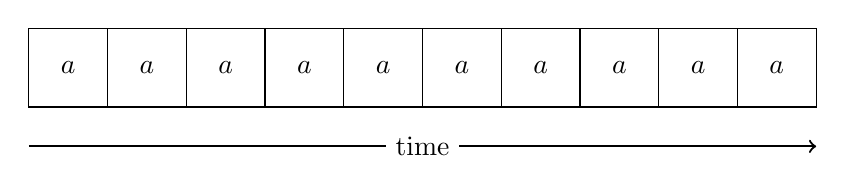
\begin{tikzpicture}[node distance=1cm]
            % Draw 10 boxes horizontally.
            % We give each box a fixed size so that we know its boundaries.
            \foreach \i in {0,...,9} {
                \node[draw, rectangle, minimum width=1cm, minimum height=1cm] (box\i) at (\i,0) {$a$};
            }

            % Draw an arrow below the boxes.
            % Here we start a bit to the left of the first box and end a bit to the right
            % of the last box so that the arrow spans across all boxes.
            \draw[->, thick] (-0.5,-1) -- (9.5,-1)
                node[midway, fill=white]{time};
        \end{tikzpicture}
    \end{center}

    If a time interval $a$ passes with no beads produced, this gives enough time for beads to
    propagate to nodes and be incorporated into a braid. This {\it statistically} defines a
    ``cohort''.

    The probability that $k=0$ beads are produced is $P(t, 0) = e^{-a\lambda x}$.

\end{frame}
%===============================================================================
\begin{frame}{Braid Statistics (II): Expectation Value and Variance}
    The number of cohorts in a time window also Poisson distributed with mean $\mu_C = P(t,
    k=0)\mu_B$. We can then form the expectation value for the number of beads in $N_C$ cohorts:

    \begin{equation}
        \mathbb{E}\left[\frac{N_B}{N_C}\right] =
        \mathbb{E}\left[\frac{T_C}{T_B}\right] =
        \lambda x \mathbb{E}[T_C]
        = 1 + a\lambda x e^{a\lambda x}
        %\qquad {\rm where} \qquad
        %\overset{\displaystyle T_B = T/N_B}{T_C = T/N_C}
    \end{equation}
    where
    \begin{equation}
        \mathbb{E}[T_C] = \frac{1}{\lambda x} + a e^{a\lambda x}
    \end{equation}
    and the variance is
    \begin{equation}
        {\rm Var}\left[\frac{N_B}{N_C}\right] = \frac{\mu_B}{\mu_C^2} + \frac{\mu_B^2}{\mu_C^3}
    \end{equation}
    These are the {\it exact} behavior of a mining network (including bitcoin!) at constant hashrate
    $\lambda$ and latency $a$.
\end{frame}
%===============================================================================
\begin{frame}{Braid Statistics (III): Target Difficulty}
    The location of the minimum in $T_C$ is given by
    \begin{equation}
        \frac{\partial T_C}{\partial x}=0
        \qquad
        \implies
        \qquad
        x = x_0 = \frac{2 W\left(\frac12\right)}{a\lambda} \simeq \frac{0.7035}{a \lambda}
    \end{equation}
    where $W(z)$ is the Lambert W function (the solution to $z = W e^W$). We can plug this into
    $N_B/N_C$ to obtain
    \begin{equation}
        \left.\frac{N_B}{N_C}\right|_{x_0} = 1 + \frac{1}{2W(\frac12)} \simeq 2.4215
    \end{equation}
    at this minimum, the mean cohort time in units of $a$ is
    \begin{equation}
        \frac{T_{C,min}}{a} = \frac{1}{a\lambda x_0} + e^{a\lambda x_0} =
            \frac{1}{2 W(\frac12)} + \frac{1}{4 W(\frac12)} \simeq 3.44
    \end{equation}
    This represents having the {\it most-frequent} graph cuts and is {\it independent of
    timestamps}.

\end{frame}
%===============================================================================
\begin{frame}{Braid Simulations I}
    \begin{tikzpicture}[overlay, remember picture]
    \node[anchor=center] at (current page.center) {
        
\includegraphics[scale=0.44]{T_C_x.png}
    }
    \end{tikzpicture}
\end{frame}
%===============================================================================
\begin{frame}{Braid Simulations II: Beads within 7 cohorts}
        \includegraphics[scale=0.30]{NB\_NC7.png}
\end{frame}
%===============================================================================
\begin{frame}{Braid Summary}
    What's going on here?

    \begin{itemize}
        \item We're using measured latency $a$ as a {\it clock}
        \item This is extremely resistant to manipulation
        \item We can't measure the hashrate $\lambda$ or latency $a$ without timestamps, but we
            don't need to.
        \item Instead we measure the {\it product} $a\lambda$ and adjust to it.
        \item By targeting the most-frequent graph cuts, we have a parameter free target for our
            difficulty adjustment

    \end{itemize}
\end{frame}
%===============================================================================
\section{Beads (Shares)}
\subsection{Beads (Shares)}
\begin{frame}{Shares and Weak Blocks}
    \begin{itemize}
        \item Beads (shares) are ``weak blocks'':they may not meet bitcoin's difficulty target $x_b$
            but meets some lesser difficulty target $x$.
        \item A Bead (share) is a {\it full bitcoin block} including transactions
        \item Pool members need to know with {\bf certainty} that other beads {\it could have been}
            bitcoin blocks had they met the target.
        \item Beads need to be {\it small} and quick to validate
        \item How do you get beads to be small?
            \begin{itemize}
                \item[$\Rightarrow$] by omitting transactions and the coinbase!
            \end{itemize}
        \item How do you validate something you omitted?
            \begin{itemize}
                \item[$\Rightarrow$] by committing to transactions and {\it deterministically
                    computing} the template based on previously-seen data
            \end{itemize}
    \end{itemize}
\end{frame}
%===============================================================================
\begin{frame}{Bead (Share) Structure}
\lstinputlisting[language=Rust]{bead.rs}
\lstinputlisting[language=Rust]{committedmetadata.rs}
\lstinputlisting[language=Rust]{uncommittedmetadata.rs}
\begin{itemize}
    \item We {\it compute} the coinbase transaction and block template independently on each node
        in order to validate a bead
\end{itemize}
\end{frame}
%===============================================================================
\begin{frame}{What's a Committed Mempool?}
    \begin{itemize}
        \item A restricted, release-tagged instance of bitcoind: no network access communicates over
            IPC, used only for its mempool
        \item Goal is to {\it prevent} block template outsourcing
        \item Every bead has an associated committed mempool implied by its parents.
        \item All transactions not yet mined in all ancestors are already in its committed mempool.
        \item Add the 2-5 transactions committed by this bead.
        \item Compute block template with any {\it deterministic} algorithm.
    \end{itemize}
\end{frame}
%===============================================================================
\begin{frame}{Advantages of a Committed Mempool}
    \begin{itemize}
        \item ALL Transactions are fully validated
            \begin{itemize}
                \item[$\Rightarrow$] All nodes know with confidence that all {\it other} beads are
                    not going to withhold blocks or generate orphans
            \end{itemize}
        \item ALL Nodes broadcast blocks as soon as they see the Bead
            \begin{itemize}
                \item[$\Rightarrow$] Impact of low bandwith or high latency nodes is removed
            \end{itemize}
        \item Transaction selection is a legal liability and no one wants to do it. Ethereum has
            only MEVil and Compliant miners.
            \begin{itemize}
                \item[$\Rightarrow$] Solve this problem by making {\it everyone} do it
            \end{itemize}
        \item Beads are {\it small} $\sim 20{\rm kb}$ so don't cause huge latency problems
        \item Most of the data for block validation is already known and re-usable.
    \end{itemize}
\end{frame}
%===============================================================================
\begin{frame}{Share Value}
    The fundamental unit of reward in Bitcoin is sha256d hashes computed. This is ``work''. But
    because of difficulty targeting, we need to allow shares to have different amounts of work.

    \vspace{0.2cm}

    Version 1 will use a full-proportional version of PPLNS.
    \begin{itemize}
        \item Expire old shares (window based on time and/or or work)
        \item Beads with very large cohorts can't pay everyone: large cohorts are an orphan risk.
            \begin{itemize}
                \item[$\Rightarrow$] Sort beads based on:
                    \begin{itemize}
                        \nitem simple sum of descendant work
                        \nitem simple sum of ancestor work
                        \nitem hash value (``luck'')
                    \end{itemize}
                \item[$\Rightarrow$] For $N_B \gsim 20$, lowest work beads won't
                    be rewarded
            \end{itemize}
        \item We're researching something better. PPLNS sucks.
    \end{itemize}
\end{frame}
%===============================================================================
%\section{Consensus}
%\subsection{Difficulty Retarget Algorithm}
%\begin{frame}{Consensus on a Directed Acyclic Graph (braid) }
%    Allowing blocks to have multiple parents creates a:
%    \begin{description}
%        \nitem[Directed] Blocks have parents, parents cannot refer to children
%        \nitem[Acyclic]  A cycle is cryptographically impossible
%        \nitem[Graph]    Structure is non-linear (no ``height'')
%    \end{description}
%    \vspace{0.5cm}
%    %Fun facts about DAGs
%    \begin{itemize}
%        \nitem A DAG can be {\it partial ordered} in linear time.
%        \nitem We have to make a restriction relative to a more general dag, so
%        I'm going to name this data structure a {\it braid}.
%        %\nitem \FIXME{foo}
%        %\nitem Orphans can be eliminated entirely
%    \end{itemize}
%\end{frame}
%===============================================================================
%\begin{frame}{Braid Terminology}
%  \begin{center}
%  \includegraphics[scale=0.7]{braid}
%  \end{center}
%  \begin{description}[Sibling]
%      \nitem[Braid]    A Directed Acyclic Graph having no {\it incest}
%      (no triangles)
%      \nitem[Bead]     Analog of Bitcoin's blocks (green circles)
%      \nitem[Sibling]  A {\it bead} that cannot be partial ordered relative to myself: the pairs
%                      (B,C) and (E,F)
%      \nitem[Incest]   A parent that is simultaneously an ancestor of another parent
%                      ({\color{red} disallowed})
%  \end{description}
%\end{frame}
%===============================================================================
%\begin{frame}{Our Approach}
%    \begin{itemize}
%        \nitem ALL beads presenting a valid proof-of-work hash receive
%        \nitem Because of {\it selfish mining}\footnote{Eyal, Sirer, {\rm arXiv:1311.0243}} we will
%        incentivize miners to quickly transmit beads
%
%        \nitem Because GHOST\footnote{Sompolinsky, Zohar, {\rm ia.cr/2013/881}}
%            worsens some attacks, we will require that {\it parents must not
%            contain conflicting transactions}
%
%        \nitem Allow all of these to be decided per-node:
%        \begin{itemize}
%            \nitem Bead time; Bead target difficulty; Bead size
%        \end{itemize}
%
%        \nitem Assume Braids will be a parallel, faster layer to Bitcoin blocks:
%        \begin{itemize}
%            \nitem Beads will be constructed such that they are valid Bitcoin blocks, if they meet
%                bitcoin's difficulty target.
%        \end{itemize}
%
%        \nitem Publish beads {\it ex-post-facto} because knowing who the current leader is
%            (Bitcoin-NG\footnote{Eyal, Gencer, Sirer, Renesse, {\rm arXiv:1510.02037}}) opens a new
%            vulnerability
%
%    \end{itemize}
%\end{frame}
%===============================================================================
%\begin{frame}{Let's Simulate!}
%    Let's build a ``toy model'' of the Bitcoin network.
%    \begin{itemize}
%        \item 25 node network
%        \item 4 connections per node
%        \item Nodes randomly distributed on the surface of (the Earth)
%        \item Inter-node latencies decided by arc distance on sphere
%    \end{itemize}
%    Python code available at
%    \begin{center}
%        {\tt http://github.com/mcelrath/braidcoin}
%    \end{center}
%
%    Another ``toy model'' for simulation is Simbit (javascript)
%    \begin{center}
%        {\tt https://github.com/ebfull/simbit}
%    \end{center}
%\end{frame}
%===============================================================================
%\begin{frame}{Cohort Time vs Difficulty}
%    \includegraphics[scale=0.4]{fastest_cohort}
%\end{frame}
%===============================================================================
%\begin{frame}{Cohort Time vs Difficulty}
%    \includegraphics[scale=0.4]{fastest_cohort2}
%\end{frame}
%===============================================================================
%\begin{frame}{Analysis}
%    There exists a {\it fastest possible cohort time!}
%    \begin{overprint}
%        \onslide<1>\includegraphics[scale=0.4]{thinbraid}
%        \onslide<2>\includegraphics[scale=0.4]{thickbraid}
%    \end{overprint}
%    \begin{overprint}
%        \onslide<1>
%            \begin{itemize}
%                \item HIGH difficulty (blockchain limit - LEFT side of graph)
%                \item Beads are produced so rarely that they can almost always
%                    be ordered into a chain.
%            \end{itemize}
%        \onslide<2>
%            \begin{itemize}
%                \item LOW difficulty (braid limit - RIGHT side of graph)
%                \item Beads are produced so fast that there's almost always one in
%                    propagating through the network!
%                \item Poisson nature of mining makes finding a cohort exponentially
%                    less likely
%            \end{itemize}
%    \end{overprint}
%\end{frame}
%===============================================================================
%\begin{frame}{Difficulty Target I}
%    The curve resulting from this simulation is extremely well approximated by
%    $$
%    T(x) = \frac{1}{\lambda x} + a e^{a \lambda x}
%    $$
%    %\hline
%    \begin{columns}[T]
%      \begin{column}{6.5cm}
%          \begin{description}[xxx] % Argument is max width of item argument
%              \nitem[$T$] Cohort time
%              \nitem[$\lambda$] Hash rate (hashes per second)
%          \end{description}
%      \end{column}
%          \vline
%          \begin{column}{6cm}
%              \begin{description}[xxx]
%                  \nitem[$x$] Target hash value
%                  \nitem[$a$] Network ``size'' parameter (in seconds)
%              \end{description}
%          \end{column}
%    \end{columns}
%
%    Let's approximate this in the blockchain limit $x\to 0$:
%    $$
%    T(x) = \frac{1}{\lambda x} + a + \mathcal{O}(x)
%    $$
%    the quantity $a$ is the {\it increase in effective block time} due to network
%    latency effects.  This is to say that the actual cohort time is slightly
%    longer than expected from the hashrate.
%
%    %$a$ is the orphan rate, or ``miner utilization''.
%\end{frame}
%===============================================================================
%\begin{frame}{Difficulty Target II}
%
%    The parameter $\lambda$ is the hash rate and can be obtained along with $a$:
%    $$
%    \lambda = \frac{N_B}{x T_C N_C}; \qquad a = T_C W\left(\frac{T_C}{T_B} - 1\right)
%    $$
%    where $N_B$ is the number of beads and $N_C$ is the number of cohorts.  $W(z)$ is the
%    {\it Lambert W function}\footnote{\tt
%    https://en.wikipedia.org/wiki/Lambert\_W\_function}.
%    With these in hand we can compute the location of the minimum
%    $$
%    x_0 = \frac{2 W\left(\frac12\right)}{a \lambda} = \frac{0.7035}{a\lambda}
%    $$
%
%    This is relatively independent of network topology.
%
%\end{frame}
%===============================================================================
%\begin{frame}{Analysis IV}
%    \begin{block}{}
%        \begin{center}
%        We can target the {\it fastest possible} block time!
%        \end{center}
%    \end{block}
%    10 minutes is arbitrary, and slow.
%    \vspace{0.5cm}
%
%    We can have a {\bf zero parameter retarget algorithm}: instead of targeting
%    a fixed block time, targets the fastest possible block time.  Evaluating the
%    above for the Bitcoin network, which has had an orphan rate of 1.16
%    orphans/day on average over the last 2 years with a block time of $600$s, we
%    find that $a=4.79$s and the cohort time at the minimum is $11.64$s.
%    \vspace{0.5cm}
%
%    By targeting the fastest block time, we automatically compensate for network
%    topology changes!
%\end{frame}
%===============================================================================
%\begin{frame}{Analysis V}
%    The network cannot measure time more accurately than $a$.  This implies:
%    \begin{itemize}
%        \item The network cannot make state transitions faster than $a$
%        \item The network cannot change difficulty faster than $a$
%        \item The network cannot change rewards faster than $a$
%    \end{itemize}
%
%    $\therefore$ let us consider allowing a {\it range} of difficulties and
%    rewards that are acceptable!
%    \begin{itemize}
%        \item[$\delta x$] acceptable range of targets
%        \item[$\delta R$] acceptable range of rewards
%    \end{itemize}
%\end{frame}
%===============================================================================
\section{Future Work}
\subsection{Future Work}
\begin{frame}{Miner-Selected Difficulty and Sub-Pools}
    \begin{itemize}
        \item As long as the miners chosen difficulty is $x_b < x < x_0$ there's
            nothing wrong with allowing miners to choose their own, since we
            know how to add work.
        \item Braidpool will choose your difficulty for you such that all miners have the same {\it
            variance}. This cannot be enforced by consensus.
        \item Miners too small to achieve constant variance will be grouped into
            a {\it sub-pool}, which:
            \begin{itemize}
                \item has outputs in the parent pool as the outputs managed by the sub-pool
                \item has an independent Braid from the parent pool
            \end{itemize}
    \end{itemize}
\end{frame}
%===============================================================================
%\subsection{SSDW}
%\begin{frame}{Conflict Resolution: Simple Sum of Descendant Work}
%    For braids having siblings (diamond-like and higher-order structures) where
%    conflict resolution is important will use the Simple Sum of Descendant Work
%$$
%    w_{\rm SSDW} = \sum_{i \in \rm descendants} w_i = \sum_{i \in \rm
%    descendants} \frac{1}{x_i (1-P_{\ge 2}(T_{C,i}))}
%$$
%\begin{itemize}
%    \item Only work within a cohort matters
%    \item In the event of a tie, the smaller hash (``luck'') is used.
%    \item We only need conflict resolution if Braidpool has its own
%        transactions.
%    \item Graph structure is manipulable at zero cost, so we ignore it
%\end{itemize}
%
%
%\end{frame}
%===============================================================================
%\section{Payouts}
%\subsection{Payouts}
%\begin{frame}{Payout Update}
%    From the Eltoo paper (Decker, Russell, Osuntokun):
%    %\includegraphics[scale=0.18]{eltoo.png}
%    \begin{itemize}
%        \item $T_{u,i}$ takes previous $T_{u,i-1}$ output and a new coinbase as
%            input (optimistic case, single Schnorr signature)
%        \item $T_{s,i}$ is the UHPO transaction tree (spent via tapscript)
%    \end{itemize}
%\end{frame}
%===============================================================================
%\begin{frame}{Payout Signing}
%    \begin{itemize}
%        \item Each payout update requires two keys: the Update Pubkey (P2TR) and
%            the Settlement Pubkey (in a tapscript).
%        \item These keys are generated by the distributed key generation phase
%            of FROST. All miners who successfully mined past blocks hold
%            FROST keyshares.
%        \item We may combine MuSig2 and FROST and use ROAST as well. (TBD)
%        \item After a bitcoin block is found, a FROST/ROAST signing ceremony is
%            kicked off among signing miners, for both the Update and Settlement
%            transactions, for the most recent unspent Braidpool coinbase at
%            least 100 blocks old.
%    \end{itemize}
%\end{frame}
%===============================================================================
%\begin{frame}{Settlement Tx: Unspent Hasher Payment Output}
%    \begin{columns}[T]
%        \begin{column}{6cm}
%            \begin{itemize}
%                \item The UHPO ``settlement'' transaction fans out and pays
%                    everyone
%                \item This UHPO transaction is the analog of the ``adversarial
%                    close'' in Lightning
%                \item It is only broadcast in the case of catastrophic failure
%                    or shutdown of Braidpool
%                \item Management of this transaction is the analog of the ``UTXO
%                    Set'' for Braidpool.
%            \end{itemize}
%        \end{column}
%        \begin{column}{6.5cm}
%            %\includegraphics[scale=0.3]{UHPO.png}
%        \end{column}
%    \end{columns}
%\end{frame}
%===============================================================================
\begin{frame}{Financial Instruments}
    \begin{itemize}
        \item We do not directly create any instant-payout (Lightning-like)
            method, instead we envision hashers trading shares for BTC
        \item Professional market makers and risk-taking trading firms would buy
            shares on centralized exchanges or via atomic swaps. (This is
            outside the scope of Braidpool, but enabled by it)
        \item With both shares (per epoch) and BTC as instruments, private
            hashrate derivative contracts can be created.
        \item Pools are currently doing this risk management function, and might
            continue to do so atop braidpool, along with their other services
            (management, monitoring, financing)
    \end{itemize}
\end{frame}
%===============================================================================
\section{Conclusions}
\subsection{Conclusions}
\begin{frame}{General Timeline}
    \begin{itemize}
        \item Braidpool V1: summer 2025
            \begin{itemize}
                \item Node software (Bob McElrath with Summer of Bitcoin students:
                    Abdullah Azeem, Aritra Majumder, Ansh Sharma, Mohd Zaid)
                \item Dashboard software (Bob McElrath with Summer of Bitcoin students:
                    Abhishek, David Borg, Priya Rani)
            \end{itemize}
        \item Braidpool V2
            \begin{itemize}
                \item Transactions (sending/trading shares)
                \item Latency optimization
                \item Sub-Pools
                \item Options-based payout mechanism
            \end{itemize}
    \end{itemize}
\end{frame}
%===============================================================================
\begin{frame}{Summary/Conclusions}
    \begin{itemize}
        \item All the elements are present to construct a truly trustless decentralized
            mining pool (Shares, Braid consensus, PPLNS)
        \item Demo!
    \end{itemize}
\end{frame}
%===============================================================================
%\begin{frame}{Braid Fork Example}
%    \includegraphics[scale=0.7]{fork1}
%    \begin{itemize}
%        \nitem A double-spend occurs in A and B
%        \begin{itemize}
%            \nitem[$\Rightarrow$] We must evaluate which braid has the most work
%        \end{itemize}
%        \nitem Beads in each fork reference either A or B as a parent
%        \nitem The highest-work braid will be decided by evaluating the work in
%            the combined work of all beads in the {\color{red}red} and
%            {\color{blue}blue} subgraphs.
%    \end{itemize}
%\end{frame}
%%===============================================================================
%\section{Miner Incentives}
%\subsection{Miner Incentives}
%\begin{frame}{How to Incentivize Miners}
%    Miner incentives must be aligned with correct operation of the network
%    \begin{itemize}
%        \nitem Consensus is {\it created} by the profit-maximizing miners
%        \nitem Let the {\it reward} be proportional to a miner's target difficulty
%        \begin{itemize}
%                \item[$\Rightarrow$] Miners can individually choose target and block rate based on
%                    {\it other considerations} (e.g. bandwidth)
%                \item[$\Rightarrow$] Bandwidth and CPU is now the only limiting factor for the
%                    network!
%        \end{itemize}
%        \nitem The existence of siblings/orphans means {\it we cannot decide miner coin allocation
%        until all beads are seen by all nodes}
%        \begin{itemize}
%                \item[$\Rightarrow$] Coin allocation will be calculated 100 blocks later
%        \end{itemize}
%    \end{itemize}
%    \vspace{0.2cm}
%    We will define several quantities that we will use in a new miner incentive formula (a.k.a. How
%    many bitcoins do I get?)
%
%
%\end{frame}
%%===============================================================================
%\begin{frame}{Difficulty as an assest}
%\end{frame}
%%===============================================================================
%\begin{frame}{Introducing time}
%\end{frame}
%%===============================================================================
%\begin{frame}{The Bitcoin Clock}
%    The introduction $R(t)$ requires us to keep a clock.
%
%    Let us assume each block commits to a time $t$.
%\end{frame}
%%===============================================================================
%\begin{frame}{Siblings}
%
%    A sibling {\color{ForestGreen}$S$} is an analog to Bitcoin {\it orphans}.  It is defined as
%    \begin{center}
%        \color{ForestGreen}
%        A bead that cannot be ordered to come before \\
%        or after mine using only the DAGs partial order
%    \end{center}
%    \begin{itemize}
%        \nitem Siblings are defined {\it per braid tip}
%
%        \nitem Siblings {\it must not} contain conflicting transactions
%
%        \nitem Siblings {\it may} contain duplicate transactions
%    \end{itemize}
%    \vspace{0.2cm}
%    If siblings share the same transaction, each sibling will be allocated a work-weighted fraction
%    of the tx fee.  (e.g. 2 siblings at the same target difficulty will each recieve 1/2 of the tx fee)
%\end{frame}
%%===============================================================================
%\begin{frame}{Cohort Difficulty}
%
%    The {\it cohort difficulty} {\color{ForestGreen}$D$} is the work of other miners during the
%    time window in which I was mining.  It is defined as:
%
%    \begin{center}
%        \color{ForestGreen}
%        The combined work of all beads between \\
%        my youngest parent and my oldest child.
%    \end{center}
%    \begin{itemize}
%        \nitem A miner with large cohort difficulty relative to his own is playing games or
%        following a perverse incentive
%        \begin{itemize}
%            \item Trying to steal fees by becoming everyone's sibling
%            \item Withholding blocks (children are late)
%            \item[$\Rightarrow$] Incentivizing small cohort difficulty incentivizes fast block
%                transmission
%        \end{itemize}
%    \end{itemize}
%\end{frame}
%%===============================================================================
%\begin{frame}{Cohorts and Siblings}
%    \includegraphics[scale=0.80]{cohort_sibling}
%
%    The cohort of bead B is (D,E,G) while its siblings are (D,E)
%    \\
%    Quiz:
%    \begin{overprint}
%        \onslide<1->
%        \begin{itemize}
%            \item Siblings of G?  Cohort of G?  %\onslide<2->{(B,C,D,E,F); (B,C,D,E,F,G)}
%            \item Siblings of D?  Cohort of D? %\onslide<3>{(B,G); (D)}
%        \end{itemize}
%    \end{overprint}
%\end{frame}
%%===============================================================================
%\begin{frame}{Miner Incentive Formula}
%    The miner of block $i$ receives a reward $R_i$:
%    \begin{equation*}
%        \label{eq:reward}
%        R_i = \sum_t^{T_i} f_t \frac{d_i}{D_i}
%        \left(\frac{1}{N_t}\right)
%        + C\frac{d_i}{D_i}\left(\frac{1}{N}\right) ;\qquad
%        N_t = \sum_s^{S_t}{\frac{d_s}{D_s}} ;\qquad
%        N = \sum_j^{N_c} \frac{d_j}{D_j}
%    \end{equation*}
%    \begin{overprint}
%    \onslide<1>
%        \hline
%        \begin{columns}[T]
%          \begin{column}{6.5cm}
%              \begin{description}[xxx] % Argument is max width of item argument
%                  \nitem[$i,j$] bead indices
%                  \nitem[$t$] transaction index
%                  \nitem[$d_i$] difficulty = 1/target
%                  \nitem[$D_i$] the cohort difficulty
%                  \nitem[$T_i$] number of transactions in bead $i$
%                  \nitem[$C$] block reward = 25 BTC
%              \end{description}
%          \end{column}
%              \vline
%              \begin{column}{6cm}
%                  \begin{description}[xxx]
%                      \nitem[$f_t$] Transaction fee for tx $t$
%                      \nitem[$S_t$] number of siblings containing tx $t$ ($S_t=1$ if no siblings)
%                      \nitem[$N_t$] Sum of weighted difficulty over siblings contining tx $t$
%                      \nitem[$N$] Sum of weighted difficulty over all beads (normalization)
%                  \end{description}
%              \end{column}
%        \end{columns}
%    \onslide<2>
%        This miner incentive formula is constructed such that it is:
%        \begin{itemize}
%            \nitem {\it linear} in miner difficulty $d_i$ (miners set their own target)
%            \begin{itemize}
%                \nitem For $\frac{d_i}{D_i} \ll N$ miner income is independent of target
%                \nitem Smaller $d_i$ means {\it smoother} income distribution over time
%            \end{itemize}
%            \nitem Fair (difficulty-weighted) split of fees $f_t$ among siblings
%        \end{itemize}
%    \onslide<3>
%        Consequences of this incentive structure:
%        \begin{itemize}
%            \nitem We're incentivized to {\it optimize the p2p topology} to quickly propagate blocks
%            \nitem Use of cohort difficulty $D_i$ incentivizes fast transmission of
%            blocks
%            \nitem Small miners can mine without joining pools: coinbase has many outputs (like
%            p2pool)
%        \end{itemize}
%    \end{overprint}
%\end{frame}
%%===============================================================================
%\begin{frame}{Evaluating the Best Braid}
%    The sub-braid containing the most work can be determined by estimating the hash rate
%    \begin{equation*}
%        H = \sum_i^{\rm miners} H_i
%    \end{equation*}
%    The best way to do this is using a likelihood function:
%    \begin{equation*}
%        W_\alpha(\{H_i\})=-\log L = -\log \prod_i^{\{\rm x_i\}} P_{x_i}(H_i t, k_i)
%    \end{equation*}
%    where $P_x(h,k)$ is the Poisson distribution
%    %\FIXME{more work\ldots details\ldots}
%
%    \begin{itemize}
%        \item Miners are incentivized to include all chain tips as parents
%            because it gives the sub-dag they're mining on more work.
%    \end{itemize}
%\end{frame}
%%===============================================================================
%\section{Conclusions}
%\subsection{Conclusions}
%\begin{frame}{Conclusions}
%    %A Braid instead of a blockchain has the following advantages
%    \begin{itemize}
%        \nitem Gettting rid of orphans forces us to the Braid structure.
%        \nitem Transaction volume is limited only by bandwidth and CPU!
%        \nitem Confirmation times can be {\it much} faster, limited only by the propagation time to
%        reach the entire network (e.g. the size of the Earth).
%        \nitem Algorithms are more complex, but seem to all be O(N): We don't have to solve the
%        Travelling Salesman Problem.
%        \nitem Miner income becomes much smoother and more predictable
%        \nitem Many ways to put this into bitcoin many incentive models:
%            simulation and testing is necessary.
%        \nitem Smaller miners do not have to use pools
%        \begin{itemize}
%            \item[$\Rightarrow$] mining decentralization!
%        \end{itemize}
%    \end{itemize}
%\end{frame}
%===============================================================================
%\begin{frame}{Equivalent Beads}
%    If miners can decide their own target difficulty, they can also decide what target difficulty
%    they accept as input.
%    \begin{itemize}
%        \nitem Miners within a geographic area, company, or payment processing network may choose
%        faster beads (lower difficulty) for speed
%        \nitem Miners may bundle beads into an {\it Equivalent Bead} that will be accepted by more
%        miners less frequently, by waiting for a PoW hash that satisfies a higher difficulty target
%        \nitem Because the original miners are omitted, an Equivalent Bead must have a special
%        coinbase that pays all of them
%        \nitem A bitcoin block is an example of the more general Equivalent Bead concept
%    \end{itemize}
%\end{frame}
%===================================== ==========================================
%\begin{frame}{Confirmation Times}
%    How do I know when a transaction is ``confirmed''?
%    \begin{itemize}
%        \item Satoshi's analysis still applies, and we must keep Bitcoin's payout schedule
%        \begin{itemize}
%            \item[$\Rightarrow$] Counting six bitcoin blocks is still resonable
%        \end{itemize}
%        \item Much better analyses are possible
%        \begin{itemize}
%            \item Do there exist other braid-tips with similar work?
%            \item What's the ratio of work in my braid tip and the next closest?
%            \item Has the hash power recently changed?
%        \end{itemize}
%    \end{itemize}
%    \pause
%    \begin{center}
%        \it
%        We have much more data: I'd like to see a whole class of risk evaluation methods added for
%        different users and use cases.
%    \end{center}
%\end{frame}
%===============================================================================
%\section{Simulations}
%\subsection{Simulations}
%\begin{frame}{Miner Profit}
%    \begin{itemize}
%        \item Miner income vs time: when miner builds only on his own blocks (graph)
%        \item Miner income vs time: at several target difficulties
%    \end{itemize}
%    Possible plots from Bitcoin-NG paper:
%    "Consensus Delay", "Fairness", "Mining Power Utilization", "Time to Win", "Subjective Time to Prune"
%\end{frame}
%===============================================================================
%\section{Conclusions}
%\subsection{Conclusions}
%\begin{frame}{Conclusions}
%    %A Braid instead of a blockchain has the following advantages
%    \begin{itemize}
%        \nitem Gettting rid of orphans forces us to the Braid structure.
%        \nitem Transaction volume is limited only by bandwidth and CPU!
%        \nitem Confirmation times can be {\it much} faster, limited only by the propagation time to
%        reach the entire network (e.g. the size of the Earth).
%        \nitem Algorithms are more complex, but seem to all be O(N): We don't have to solve the
%        Travelling Salesman Problem.
%        \nitem Miner income becomes much smoother and more predictable
%        \nitem Many ways to put this into bitcoin many incentive models:
%            simulation and testing is necessary.
%        \nitem Smaller miners do not have to use pools
%        \begin{itemize}
%            \item[$\Rightarrow$] mining decentralization!
%        \end{itemize}
%    \end{itemize}
%\end{frame}
%===============================================================================

\end{document}


% TODO
% Diagrams:
%   T_{s,i} UHPO fan-out
%   T_{u,i} coinbase aggregation including new coinbase input
